\subsection{Overall Model Performance}

We tested three different approaches: RAG, Moderator, and Combined, on a set of 200 medication-related questions. The outcomes were compared to a manual review, which acted as our gold standard for correctness. According to this review, 140 of the answers were considered correct and 60 were incorrect.

Looking at Figure~\ref{fig:prediction_performance_bar}, the differences between the models quickly become clear. Moderator picks up the most correct answers, with 133 true positives, and misses only 7 false negatives. However, it also produces the most false positives at 50, which means it can be too generous in what it accepts as correct. Its true negatives are low, only 9, showing it is not strict in filtering out wrong answers.

RAG finds 109 true positives and 28 true negatives. Both false positives and false negatives stand at 31, which suggests this approach sits right in the middle. RAG does not lean toward one type of error and can be seen as a neutral or balanced option.

The Combined approach is the most careful. It only accepts 104 correct answers and misses 36, so it tends to overlook good answers. On the upside, it produces the fewest false positives at 28 and the highest number of true negatives at 31. This tells us that Combined is the strictest in its standards.

\begin{figure}[ht]
  \centering
  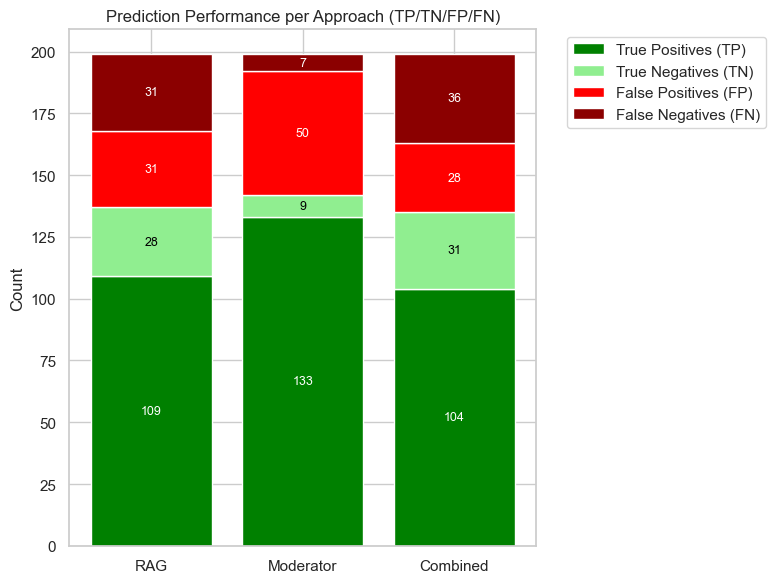
\includegraphics[width=0.95\linewidth]{figures/prediction_performance_per_approach.png}
  \caption{Prediction Performance per Approach, showing true positives, true negatives, false positives, and false negatives for RAG, Moderator, and Combined.}
  \label{fig:prediction_performance_bar}
\end{figure}

\subsection{Performance Metrics and Trade-offs}

Figure~\ref{fig:model_performance_comparison_per_metric} shows the key performance numbers for each model: precision, recall, F1 score, and accuracy. Moderator scores highest on recall at 95.0 percent, so it almost never misses a correct answer. The trade-off is that its precision drops to 72.7 percent, as it tends to let more incorrect answers through. Combined flips this pattern and is most careful in what it approves, with a precision of 78.8 percent, but its recall drops to 74.3 percent, so it lets more good answers slip by. RAG sits right in the middle, with precision and recall both at 77.9 percent.

When we look at F1 score and accuracy, Moderator comes out on top, but not by much. Its F1 score is 82.4 percent, and accuracy is 71.4 percent. RAG and Combined follow closely behind. This mix of strengths and weaknesses in each model reflects the real-world trade-offs you face when choosing a guardrail approach.

\begin{figure}[ht]
  \centering
  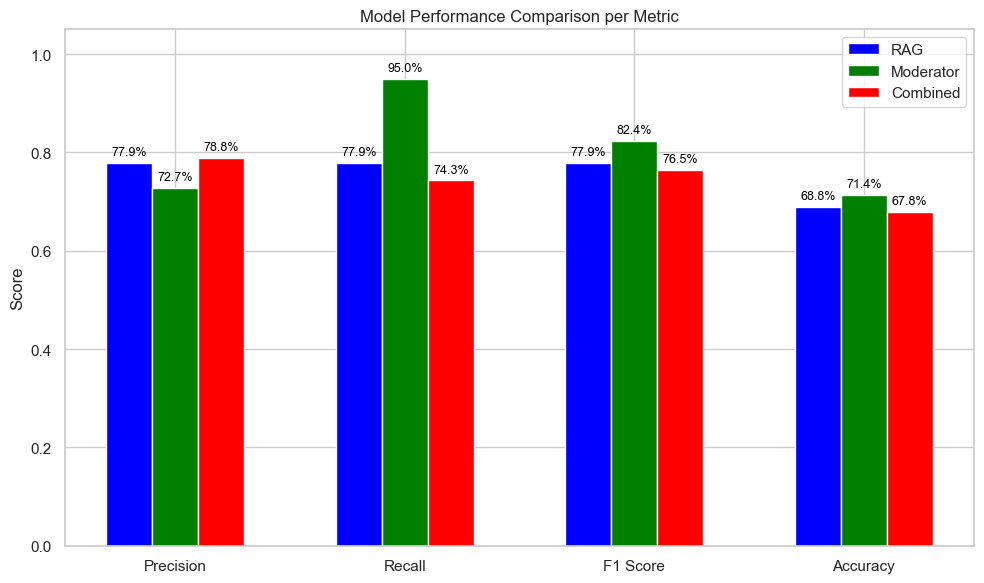
\includegraphics[width=0.95\linewidth]{figures/model_performance comparison_per_metric.png}
  \caption{Model Performance Comparison per Metric: precision, recall, F1 score, and accuracy for each model.}
  \label{fig:model_performance_comparison_per_metric}
\end{figure}

\subsection{Can Perfect Correctness Be Achieved?}

One of the main questions in this research was whether combining RAG and Moderator could guarantee perfect correctness. The short answer is no. Even the combined approach falls short. It gives 104 true positives and 36 false negatives. While it does cut down on false positives, it still misses a fair number of correct answers. No model in this study produced perfect results.

\subsection{How Was Correctness Defined?}

Throughout this project, correctness was defined using a strict set of criteria. An answer was only considered correct if it matched the manual reviewer's judgment on both the medical content and whether the medication, dosage, and indication were appropriate. Every performance metric reported here uses this definition.

\subsection{Summary}

To sum up, each model has its own personality. Moderator hardly misses any correct answers but is not picky enough, letting through a lot of false positives. Combined is picky and almost to a fault, which means it avoids false positives but also overlooks more good answers. RAG sits comfortably in the middle, with no big risks either way. None of the models manages to be perfect, so the best choice depends on what kind of error matters most for your application. Figures~\ref{fig:prediction_performance_bar} and~\ref{fig:model_performance_comparison_per_metric} offer a visual summary of these findings.

